\documentclass[12pt]{article}
\usepackage[margin=1in]{geometry} 
% \usepackage[english]{babel}
\usepackage{amsmath}
\usepackage{tcolorbox}
\usepackage{amssymb}
\usepackage{amsthm}
\usepackage{lastpage}
\usepackage{fancyhdr}
\usepackage{accents}
\usepackage{hyperref}
\pagestyle{fancy}
\setlength{\headheight}{40pt}

\hypersetup{
    colorlinks=true,
    linkcolor=blue,
    filecolor=magenta,      
    urlcolor=cyan,
    pdftitle={Overleaf Example},
    pdfpagemode=FullScreen,
  }


\newenvironment{solution}
  {\renewcommand\qedsymbol{$\blacksquare$}
  \begin{proof}[Solution]}
  {\end{proof}}
\renewcommand\qedsymbol{$\blacksquare$}

\newcommand{\ubar}[1]{\underaccent{\bar}{#1}}

% \addbibresource{./resources/references.bib}

 % add packages, settings, and declarations in settings.tex
\usepackage{wrapfig}

\title{Transforming Text Comprehension}
\author{Christian Bauer, 01560011}
\date{}

% \bibliographystyle{plain}
% \addbibresource{./resources/references.bib}

\begin{document}


\maketitle

% Report

% A report should be a 6-8 pages long document structured as a research paper, as shown below. You may modify this structure, but the suggested list is a good starting point.

\tableofcontents
    
\pagebreak

    \section{Motivation}
    \label{sec:motivation}

    % Motivation: describe the problem you are solving, explain why is it important, and provide a short summary of your methods and obtained results.

        % NLP is a hard task for computers and writing a chatbot that "understands" user input, meaning providing a satisfactory answer is a challenging task.
        % For the project, a chatbot will be implemented, which should be able to answer questions from the \emph{Stanford Question Answering Dataset} (short= \emph{SQuAD})\footnote{SQuAD source: \url{https://rajpurkar.github.io/SQuAD-explorer}}.
        % This dataset was extracted by volunteers with over 500 Wikipedia articles. 
        % Each of these articles is considered a title in the dataset and each holds numerous \emph{question-answer-sets (=QAS)}.
        % This SQuAD-dataset will be the source for the training dataset used to train the machine learning models.
        Natural Language Processing (NLP) is a hard task for computers and creating a system that is able to "comprehend" natural language to be able to provide a reasonable answer to questions is very challenging and a lot of research is done at the moment to improve NLP tasks.
        The first idea for this project was to implement a chatbot that will be build on top of a Feed Forward Neural Network (FNN).
        While researching resources for that task, a more interesting task was found, the comprehension of text with the help of deep learning.

        The task of natural language comprehension was a more challenging approach, since opposed to the chatbot using FNN that was used similar to a lookup table, finding the correct answer to a question given some context was a daring and unknown field to me.
        This comprehension is already widely used by companies such as Google, and often when you look for a topic, you get a well-defined short summary presented above all query objects.
        Creating NLP-models that are able to comprehend text at a human reader level is a goal for a long time in the computer science field and while there are already very impressive models available, this level of text comprehension is yet not achieved.
        
        For this project, the text comprehension neural networks called \texttt{BERT} is being used.
        BERT reaches impressive amounts of text comprehension in competitions such as the competition using the \emph{Stanford Question Answering Dataset (SQuAD)}.



    \section{Data}
    \label{sec:data}
    % Data: describe the data you are using in the project and provide examples. what kind of data you are using, where does it come from? what are the properties of your data, like balance, missing values, scale, etc., and what are you going to do about it? what kind of preprocessing, filtering, augmentation, or other manipulations are you applying in the project?  

        For the project, "The Stanford Question Answering Dataset (SQuAD)"\footnote{Source: https://rajpurkar.github.io/SQuAD-explorer/} will be used. This dataset was generated for reading comprehension training and the data is based on Wikipedia articles.
        There exist two versions of this dataset, \texttt{SQuAD 1.1} that holds 100,000 question-answer sets, and \texttt{SQuAD 2.0} that contains all question-answer sets from \texttt{SQuAD 1.1} and additionally also includes 50,000 question-answer sets that are unanswerable, and a modern reading comprehension system has to be able to also determine whether a question is answerable or not.


        \subsection{Example Data Element of SQuAD}
        \label{subsec:data-example}

            As an example, a section from the \texttt{Prime\_number} data chunk was taken as can be seen in figure \ref{fig:-squad-example}. On the left, the \emph{context} is shown, which is the text paragraph that contains the answer at some position.
            In the right column of the figure, the question is presented in bold letters, and the ground truth answer that is to be found is highlighted in green. \emph{Note: This is only partially represents the actual data that is provided by SQuAD.}

            \begin{figure}[h!]
                \centering
                \caption{SQuAD Example Question-Answer Set\cite{squadExample}}
                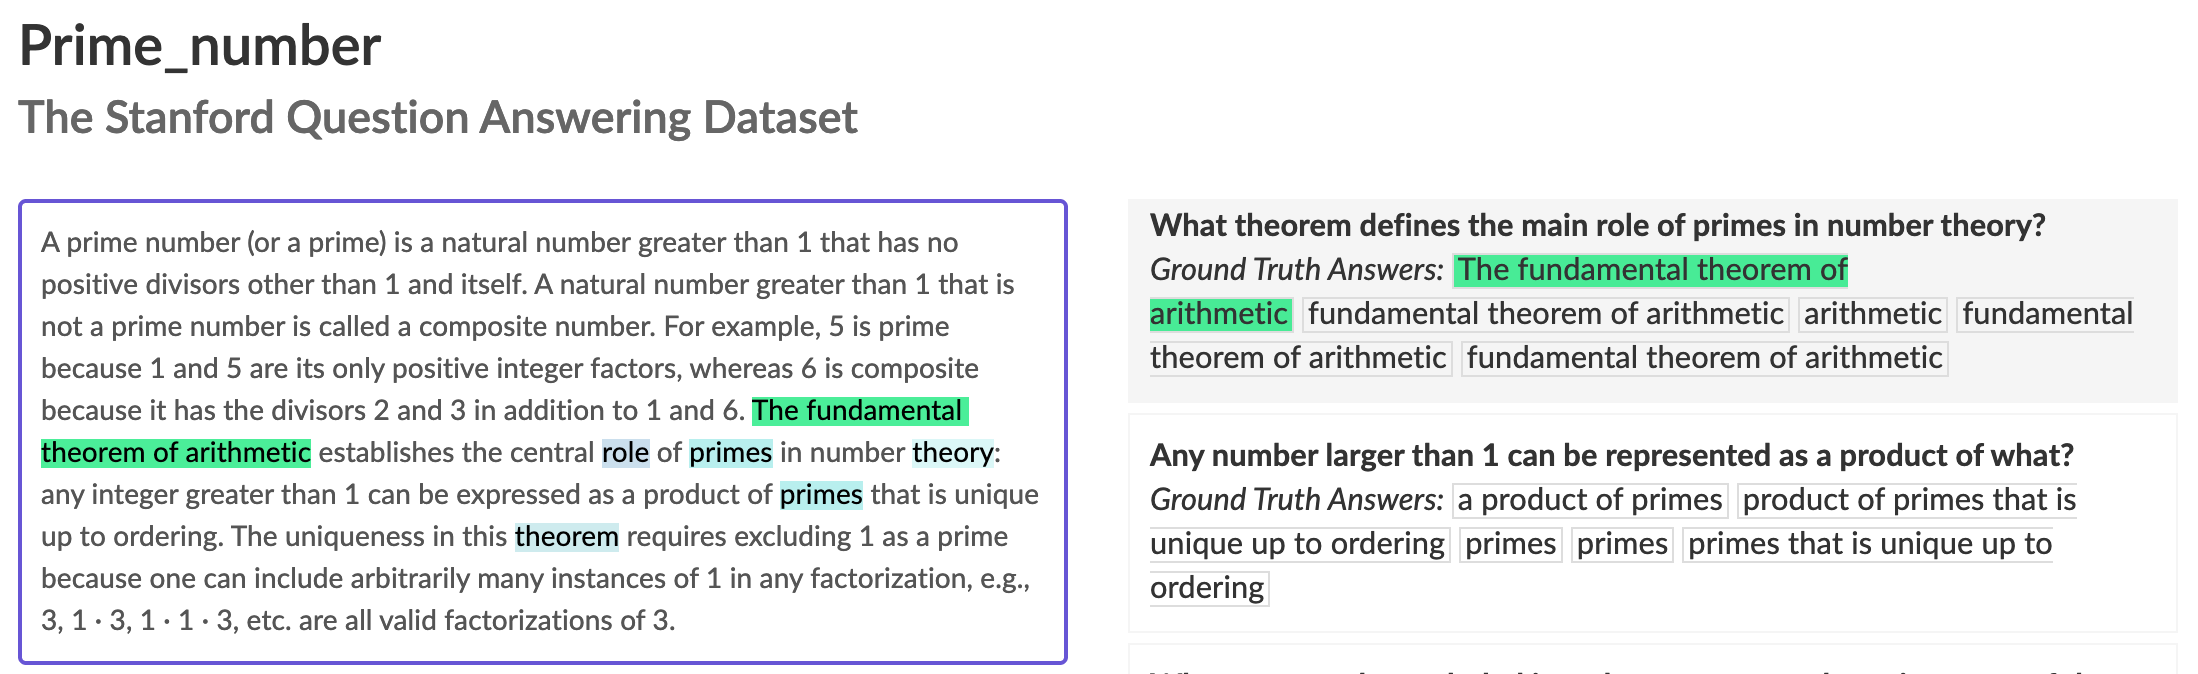
\includegraphics[width=0.95\textwidth]{figures/squad_example.png}
                \label{fig:-squad-example}
            \end{figure}

            The dataset is provided by the company \emph{Hugging Face}\footnote{URL: https://huggingface.co/}
            This company provides a vast amount of datasets and (pretrained) machine learning models. 
            Those are also used in this project and are downloaded by using the Python library \texttt{datasets} created by Hugging Face.

            \begin{figure}
                \centering
                \caption{Usage of the \texttt{datasets} library\cite[\texttt{data\_properties.ipynb}]{innerProject}}
                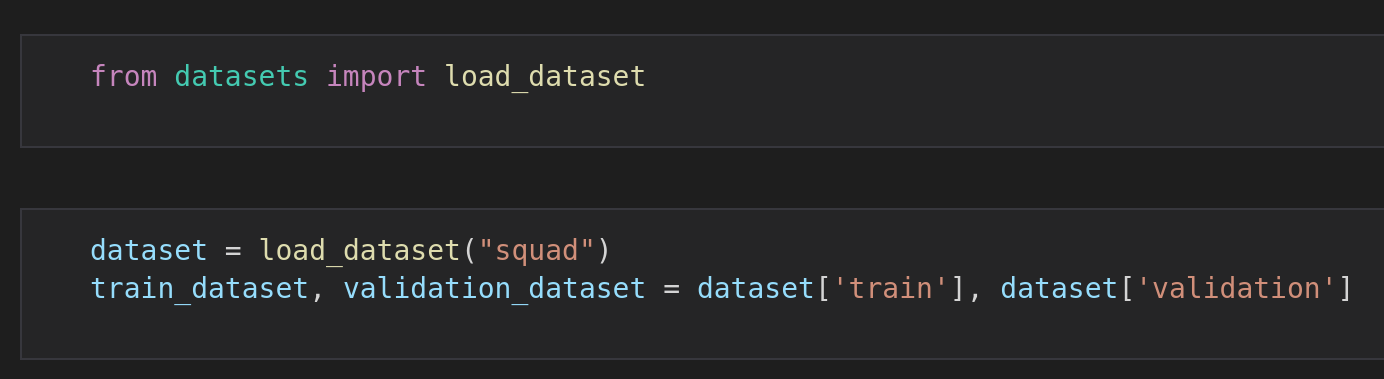
\includegraphics[scale=0.8]{figures/datasets_library.png}
                \label{fig:-datasets-library}
            \end{figure}

            With the help of the code in figure \ref{fig:-datasets-library} the train- and validation datasets can be downloaded.
            Each set consists of the following components:
            \begin{itemize}
                \item \textbf{Id:} The unique identifier of the SQuAD element.
                \item \textbf{Title:} The title of the Wikipedia entry the SQuAD element is based on.
                \item \textbf{Question:} A string containing the question the model gets asked.
                \item \textbf{Context:} A larger text sequence that contains the answer to the question.
                \item \textbf{Answer:} The part of the context, that answers the question as well as the start position of the answer in the context.
            \end{itemize}

            \begin{figure}
                \centering
                \caption{SQuAD Train Dataset Example\cite[\texttt{bert\_training.ipynb}]{innerProject}}
                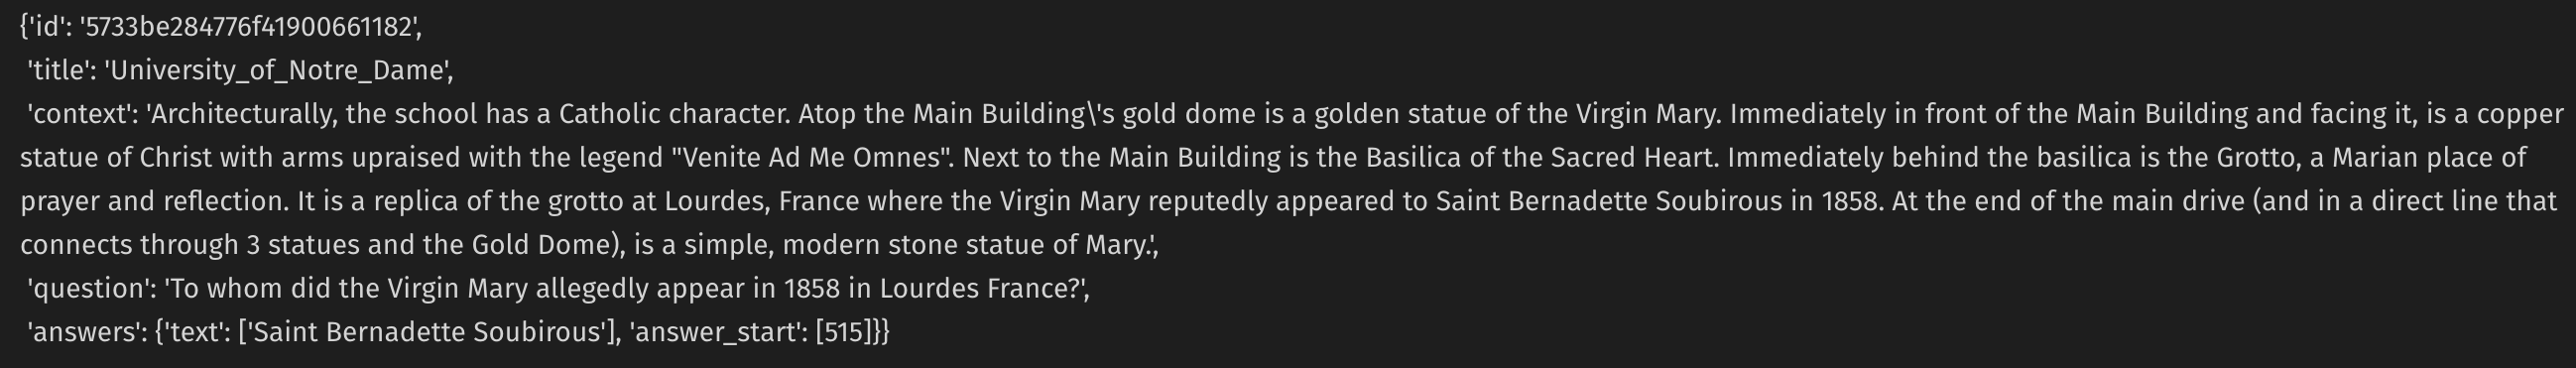
\includegraphics[width=0.99\textwidth]{figures/train_dataset_example.png}
                \label{fig:-train-dataset-example}
            \end{figure}

        \subsection{Data Properties}
        \label{subsec:-data-properties}

            The data properties were investigated with the focus of rather general values, like number of data entries in total, missing values and the balance of the dataset. All the figures used in this section are taken from the Jupyter file \texttt{data\_properties.ipynb} that can be found in the \texttt{bert\_squad} package.
            
        % TODO what are the properties of your data, like balance, missing values, scale, etc.
            \subsubsection{General Data Properties and Missing Values}
            \label{subsubsection:-data-properties---missing-values}
                The dataset consists of a total of $98169$ SQuAD elements that are split into a test dataset and validation dataset. The training dataset consists of $87599$ SQuAD elements and the validation dataset consists of $10570$.

                \begin{wrapfigure}{R}{0.5\textwidth}
                    \caption{Missing Values}
                    \begin{center}
                        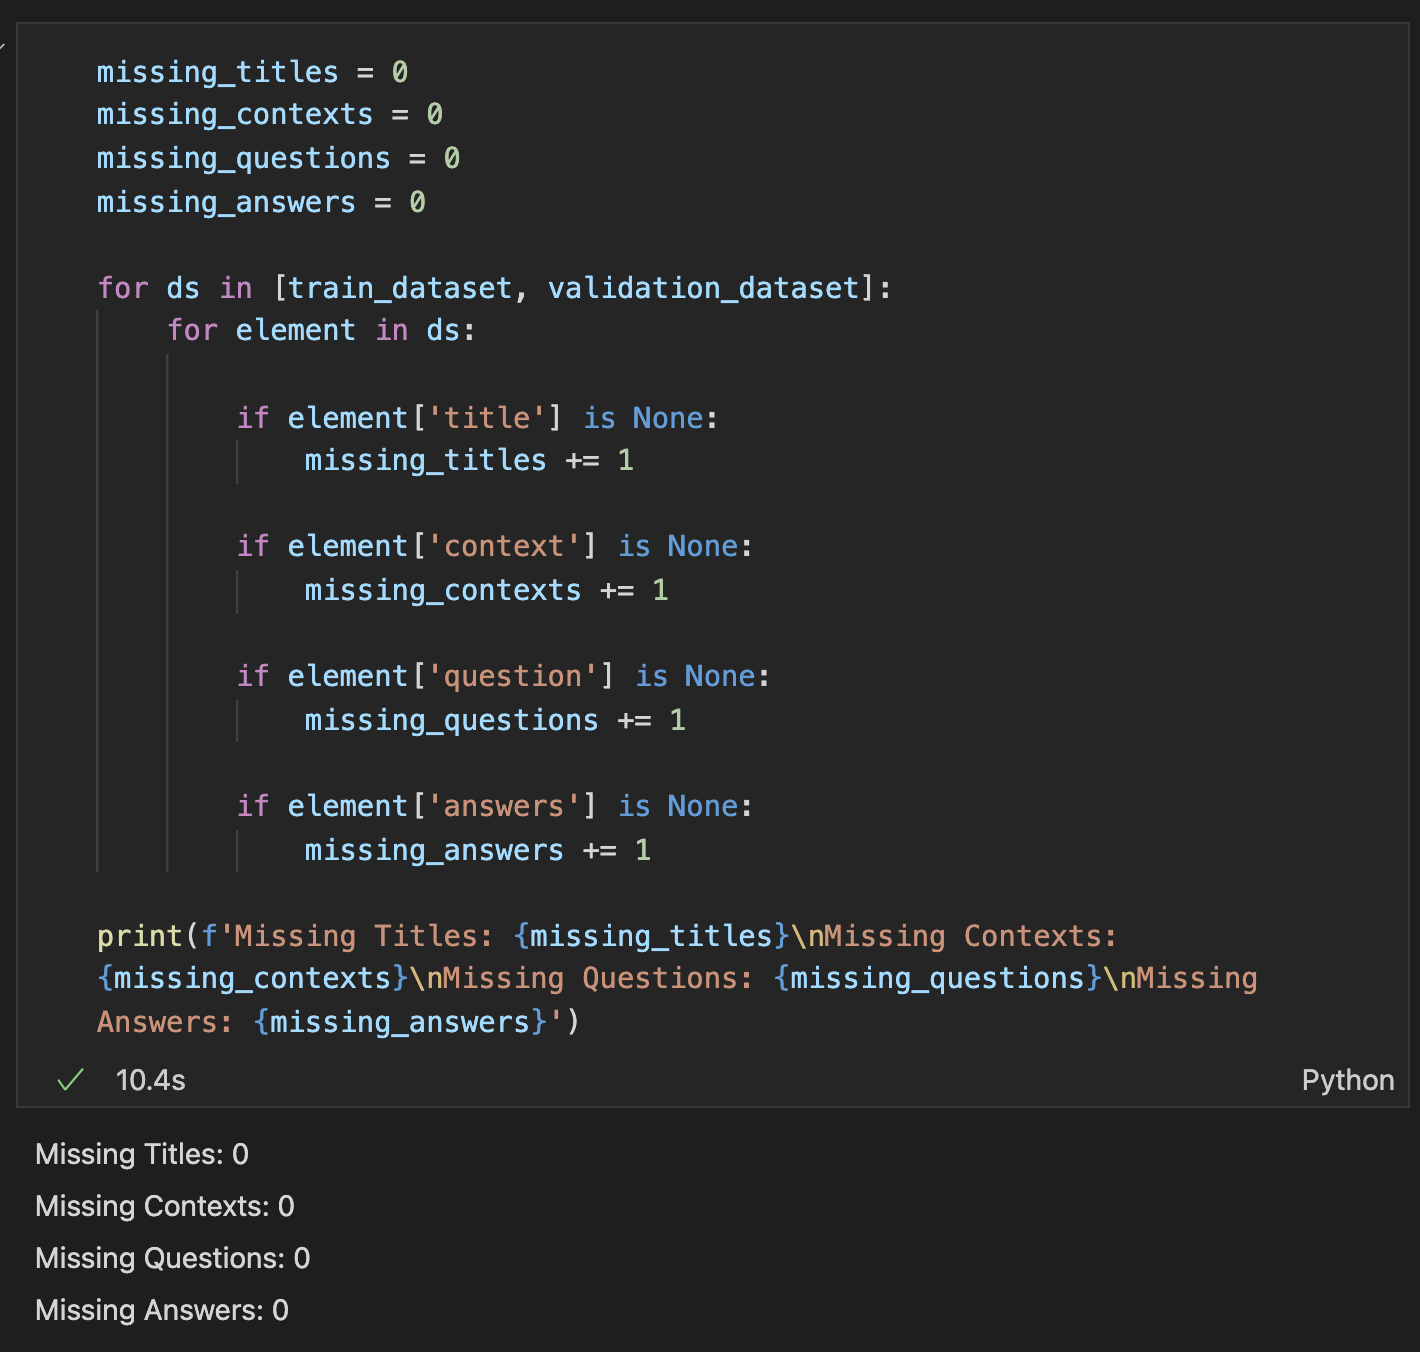
\includegraphics[width=0.49\textwidth]{figures/data_prop_no_missing_elements.png}
                    \end{center}
                    \label{fig:-data-properties---no-missing-values}
                \end{wrapfigure}

                The dataset is complete in the sense that no dataset element is missing a field value. This was tested in the Jupyter file \texttt{bert\_squad/data\_properties.ipynb} and can be seen in figure \ref{fig:-data-properties---no-missing-values}.

            
            \subsubsection{Data Balance of SQuAD}
            \label{subsubsection:-data-properties---balance-of-data}

                The dataset itself is quite unbalanced, with the maximum being a total of $817$ entries and the minimum being only $22$ Question Answer entries. 
                The mean over the entire training dataset being $198.18778$ entries per title.
                In figure \ref{fig:-data-properties---balance-of-data-barplot} a bar plot is used over all values of the training dataset to display the imbalance of the dataset visually.
                As can be seen in the graph, the number of entries for each data entry varies a lot over the overall training dataset.

                \begin{figure}[h!]
                    \centering
                    \caption{Balance of SQuAD}
                    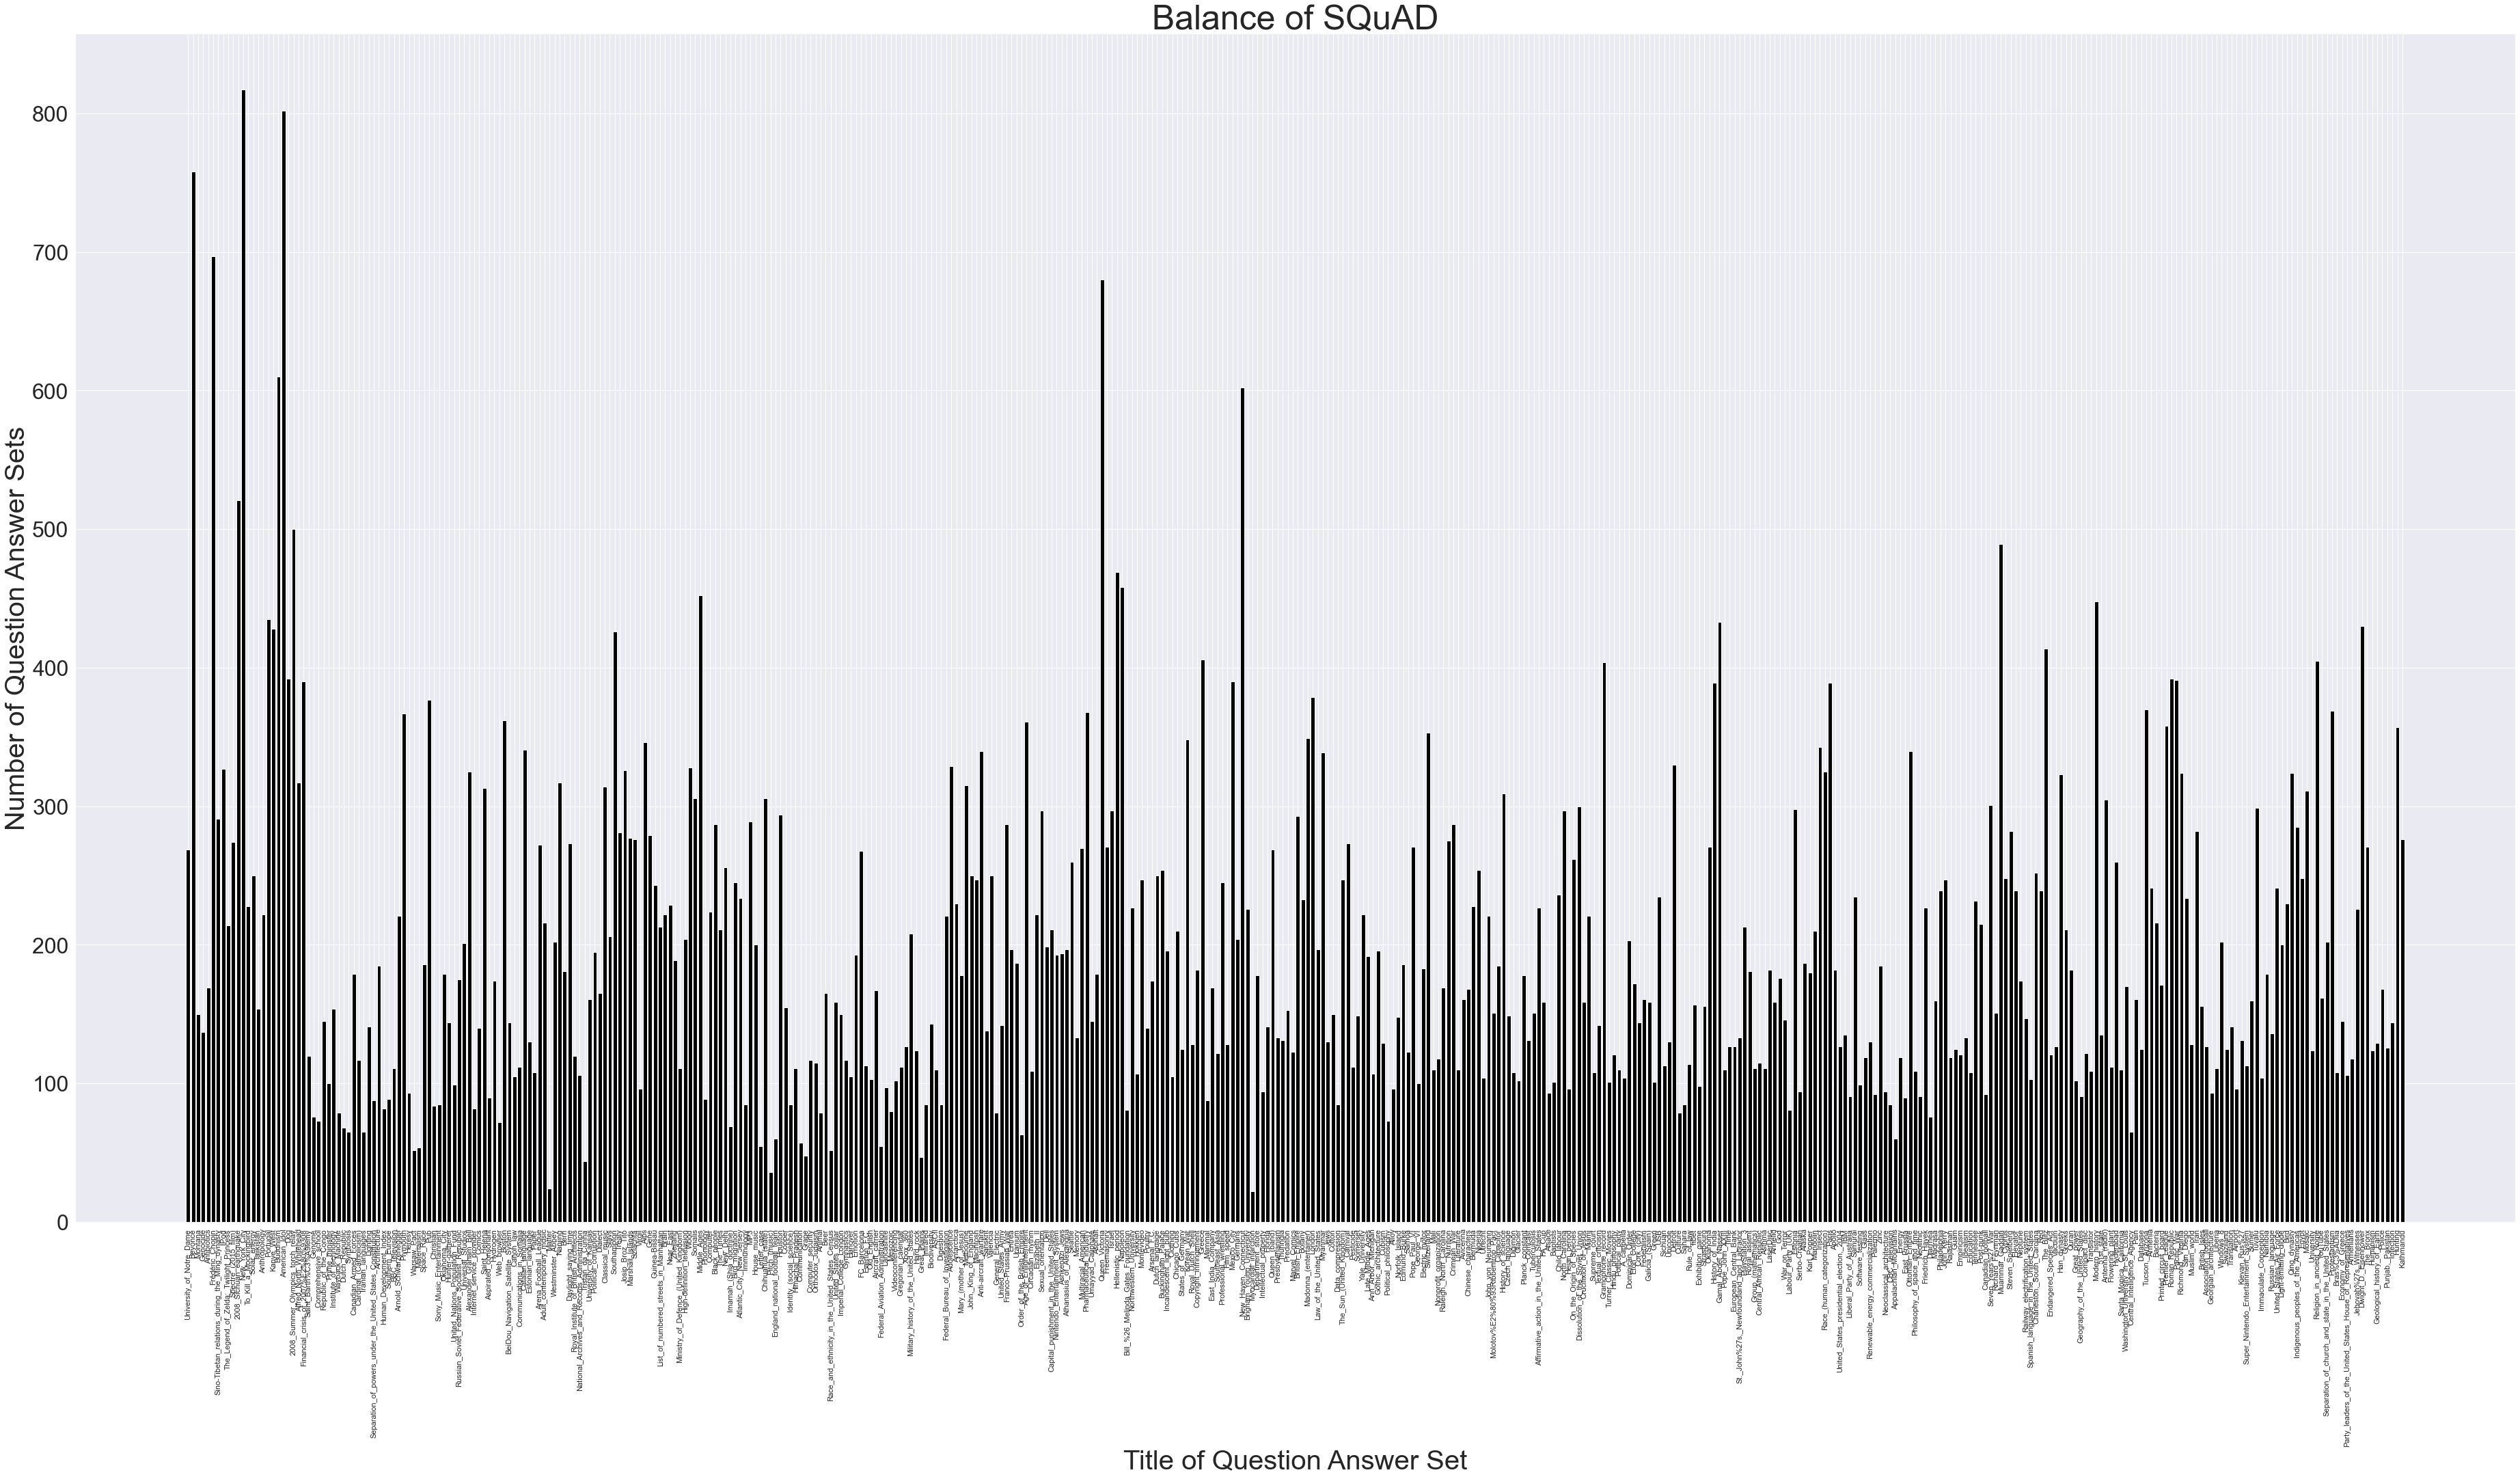
\includegraphics[width=0.95\textwidth]{figures/balance_of_squad_dataset.png}
                    \label{fig:-data-properties---balance-of-data-barplot}
                \end{figure}


            \subsubsection{Answer Position Off by One or Two Positions}
            \label{subsubsection:-data-properties---incorrect-answer-positions}

                In the used reference "How to Train Bert For Q\&A in Any Language"\cite{bertTorwardsDataScience} it was stated, that 
                some SQuAD answer positions might be off by one or two tokens, and this is corrected in the function called \texttt{add\_end\_idx} (further discussed in section \ref{section:-preparing-data-with-add-end-idx}).
                While investigating the dataset for the occurrence of such misaligned answers, none could be found. 
                The test of this was quite simple, there happens a check for a misaligned answer position inside the code, and for the investigation every SQuAD element was added to a list, and since this list was still empty after both the training-, and validation dataset were preprocessing with the \texttt{add\_end\_idx} function, no misaligned elements either exist or couldn't be found by this function. 
                This leads to the assumption, that this statement either refers to another dataset, the dataset provided by huggingface was corrected in the meantime, or that this was a wrong assumption by the author.

% \pagebreak
        \subsection{Data Preprocessing/Augmenting}
        \label{subsec:-data-preprocessing-augmenting}

            Multiple steps of data preprocessing or data augmentation were used to be able to use the dataset for the machine learning approach used. 
            Those steps are mentioned in this section according to the sequence in the \texttt{bert\_training.ipynb} they are actually used.

            \subsubsection{Preprocessing with Prepare Data Function}
            \label{subsubsec:-preparing-data-with-prep-data}
            
                \begin{wrapfigure}{r}{0.40\textwidth}
                    \caption{The Function \texttt{prep\_data}}
                    \begin{center}
                        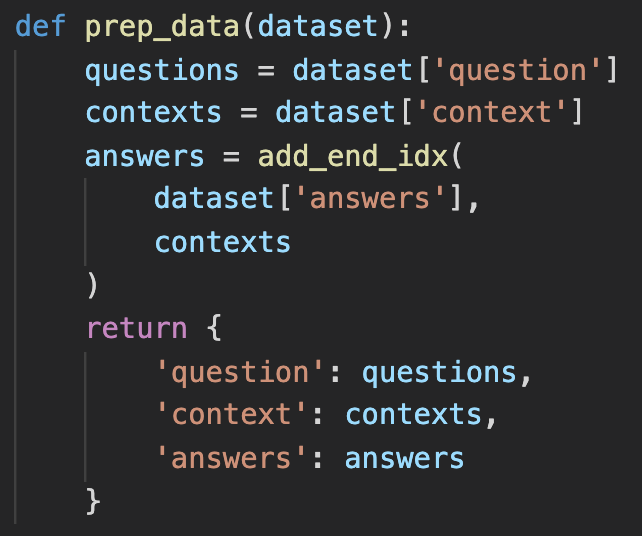
\includegraphics[width=0.3\textwidth]{figures/prep_data_function.png}
                    \end{center}
                    \label{fig:-preparing-data-with-prep-data-function}
                \end{wrapfigure}
                With the help of the function \texttt{prep\_data}, all irrelevant fields get omitted, such as \texttt{id, title}, since they will not be used in the training of the ML-model.
                This function also calls another function that is responsible for adding the answer for every question in the proper manner, so they can be used for the training. This is further explained in the section \ref{section:-preparing-data-with-add-end-idx}.
                The \texttt{prep\_data} function will be used on both the training dataset and the validation dataset before further preprocessing.


            \subsubsection{Preprocessing with \texttt{add\_end\_idx}}
            \label{section:-preparing-data-with-add-end-idx}

                The function \texttt{add\_end\_idx} is used to make later manipulations of the answer field of each SQuAD entry easier, as well as adding the inner field \texttt{answer\_end} to it, that denotes the end index position of the \emph{gold text} (gold text denotes the answer we are expecting in the context) found in the context.
                \begin{wrapfigure}{R}{0.6\textwidth}
                    \caption{The Function \texttt{add\_end\_idx}}
                    \begin{center}
                        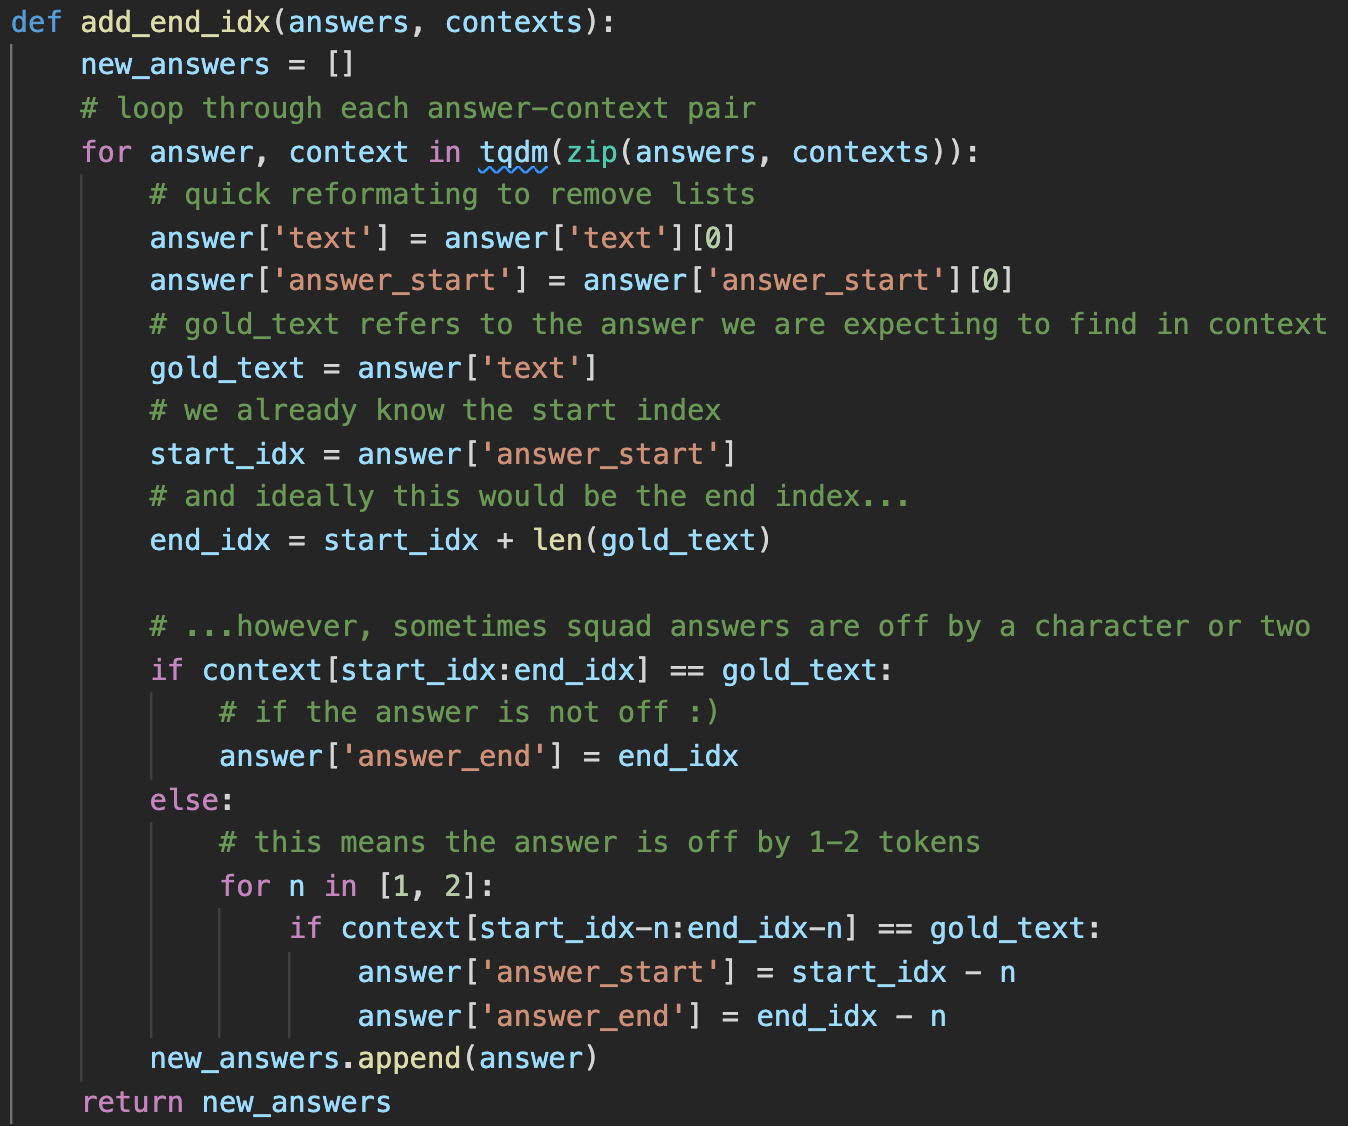
\includegraphics[width=0.5\textwidth]{figures/add_end_idx_function.png}
                    \end{center}
                    \label{fig:-data-preprocessing-augmenting---preparing-data-with-add-end-idx-function}
                \end{wrapfigure}
                The inner fields \texttt{'text', 'answer\_start'} both hold a list of data, each with one element, the first holding the answer text, the latter holding an integer element, that denotes the start position of the answer text. To make later manipulations and retrieval of those values easier, the fields simply will hold the single value of each list instead of the list with only one element.
                In the next step, the end index position of the gold text will be added, which is simply the start index position plus the length of the gold text.

                Next, with an index slice plus a check if the answer start and end index position inside the context match the gold text.
                As stated in \ref{subsubsection:-data-properties---incorrect-answer-positions}, the author of the reference "How To Train Bert Q\&A in Any Language"\cite{bertTorwardsDataScience} mentioned that the positions of the indices can be misaligned for some data entries. 
                This could not be verified with the provided code and some tests, but this part was still kept in the code in case this was referring to the SQuAD 2.0 dataset, which was not used at for now.
                After those steps, the answers given to this function will be replaced by this augmented answer dictionary.


            \subsubsection{Tokenization}
            \label{par:-data-preprocessing-augmenting---tokenization}

                To be able to feed the dataset to the ML-model BERT (see \ref{sec:-bert}), a tokenization process is necessary.
                For this the tokenizer \texttt{BertTokenizerFast} provided by the huggingface package \texttt{transformers} is used.
                This tokenizer can be used for both the \texttt{context} and \texttt{question} fields of all SQuAD entries and encodes each of them to an array of single tokens. 
                As an example, the sentence "Computer Vision research has made a giant leap since AlexNet" will be tokenized to "[CLS] computer vision research has made a giant leap since alexnet [SEP]" after decoding.
                Those encoded arrays called \texttt{input\_ids} contain special tokens required by BERT to properly understand the provided input. These arrays also contain the input ID for every word provided as an input to the tokenizer.
                This can be seen in the figure \ref{fig:-tokenizer-output-decode} in the first cell, in which the example input is tokenized and a dictionary with the field \texttt{input\_ids} contains the input IDs for every word.
                \begin{figure}[h!]
                    \centering
                    \caption{Tokenization of Input and Decoding To String \cite[\texttt{bert\_training.ipynb}]{innerProject}}
                    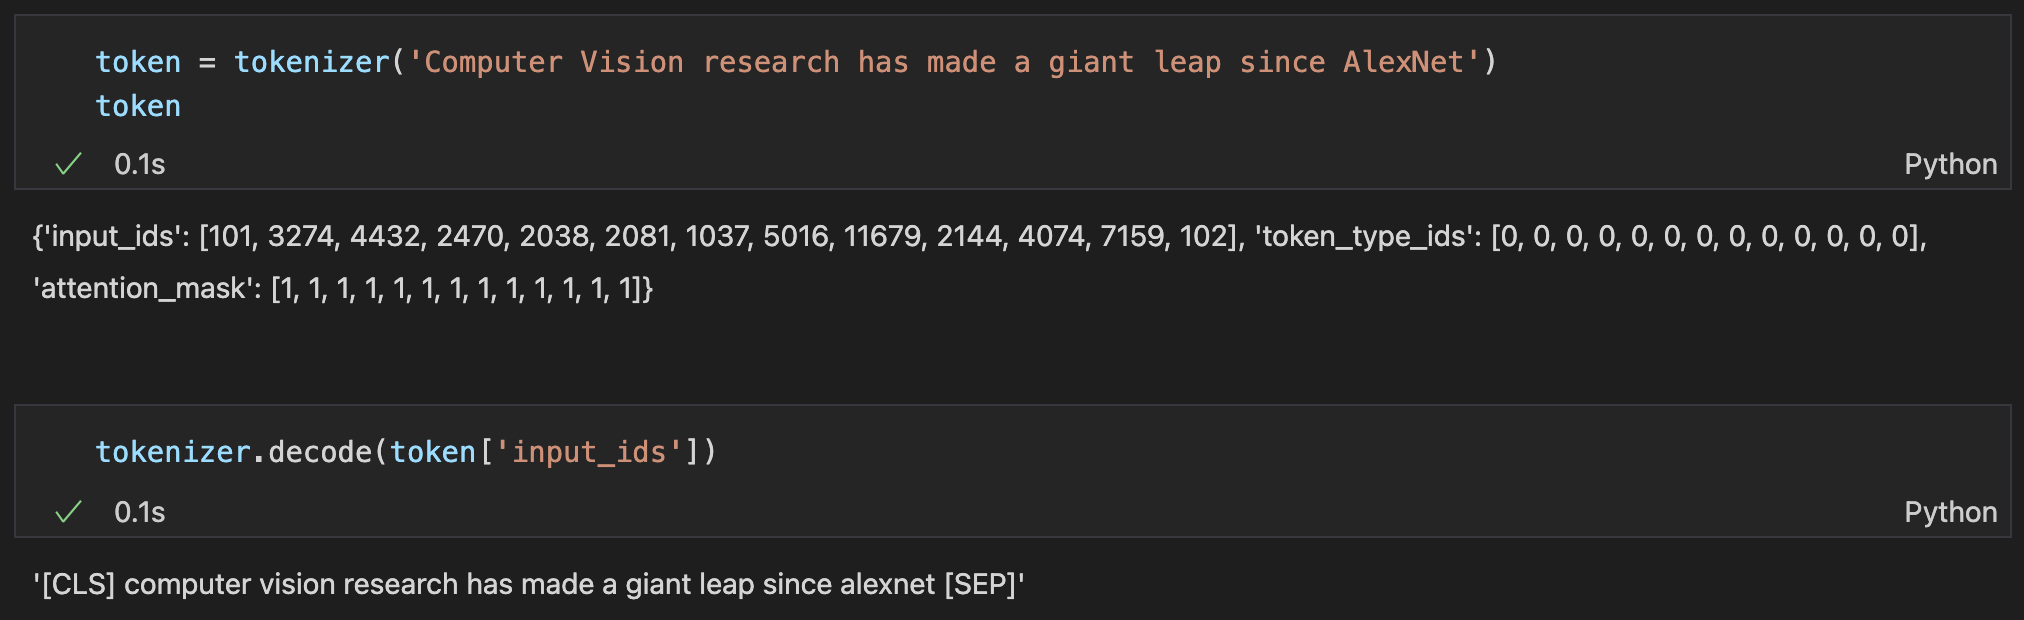
\includegraphics[width=0.95\textwidth]{figures/tokenizer_output_decode.png}
                    \label{fig:-tokenizer-output-decode}
                \end{figure}
                \emph{Note: The used tokenizer is already pretrained for the usage of text comprehension and doesn't need additional training steps.}


                \paragraph{The Classification Token}
                \label{par:-the-classification-token}

                    \texttt{[CLS]} is a special classification token and the last hidden state of BERT corresponding to this token ($h_{[CLS]}$) is used for classification tasks. \cite[Section - Model Overview]{allYouNeedBERT}


                \paragraph{The Separator Token}
                \label{par:-the-separator-token}

                    The separator token \texttt{[SEP]} has to be put at the end of a single input.
                    When a task requires more than one input such as NLI and Q-A tasks, \texttt{[SEP]} token helps the model to understand the end of one input and the start of another input in the same sequence input \cite[Section - Model Overview]{allYouNeedBERT}.


            \subsubsection{Adding Token Positions}
            \label{par:-data-preprocessing-augmenting---adding-token-positions}

                Since tokens get fed into the ML-model, the start and end positions of the tokens also need to be provided.
                This is done with the help of the function \texttt{add\_token\_positions} found in the \texttt{bert\_training.ipynb} file of the \texttt{bert\_squad} package.

\pagebreak
    \section{Theoretical Part}
    \label{sec:theoretical-part}
            
    % Theoretical part: literature overview: which models from the literature are suitable for this problem given your data and why? which algorithms can be used to train them? how these models are related to your hypothesis? present an overview of your approach: what steps are executed in the learning pipeline? which hyperparameters of the learning algorithm are available and how they can influence the results? You must show that you applied methods considered during the semester to the selected problem. Feel free to include any figures or tables helping to describe your method and compare it with others. If you use information from other sources, please cite it properly.

    
    
    \subsection{Attention}
    \label{sec:-attention}
    
    Attention is an important building block inside the Transformers model architecture (see \ref{sec:-transformers}).
    It was developed to increase the performance of encoder-decoder Recurrent Neural Network (RNN) models.
    One of the drawbacks of using encoder-decoder architectures was the fixed input vector length which will be decoded to an output at each step.
    This decoding step might result in issues, if the neural network has to decode an input that consists of long sentences, especially those longer than the ones used to train the model.

    The basic idea of Attention is that the model will try to predict an output word based on the most relevant information of the input, so it only takes parts of the given input into account instead of the whole sentence.
    This means, attention tries to give more importance to a few input words.

    Two types of attention layers are used in BERT, the "Self Attention" and the "Multi Head Attention".
    A short introduction to both concepts can be found at "Understanding Attention Mechanism: Natural Language Processing"


    
    \subsection{Transformers}
    \label{sec:-transformers}
    
    Placeholder
    
    \begin{wrapfigure}{r}{0.4\textwidth}
        \caption{The Transformer - model architecture \cite[Figure 1 on page 3]{vaswani2017attention}}
        \begin{center}
            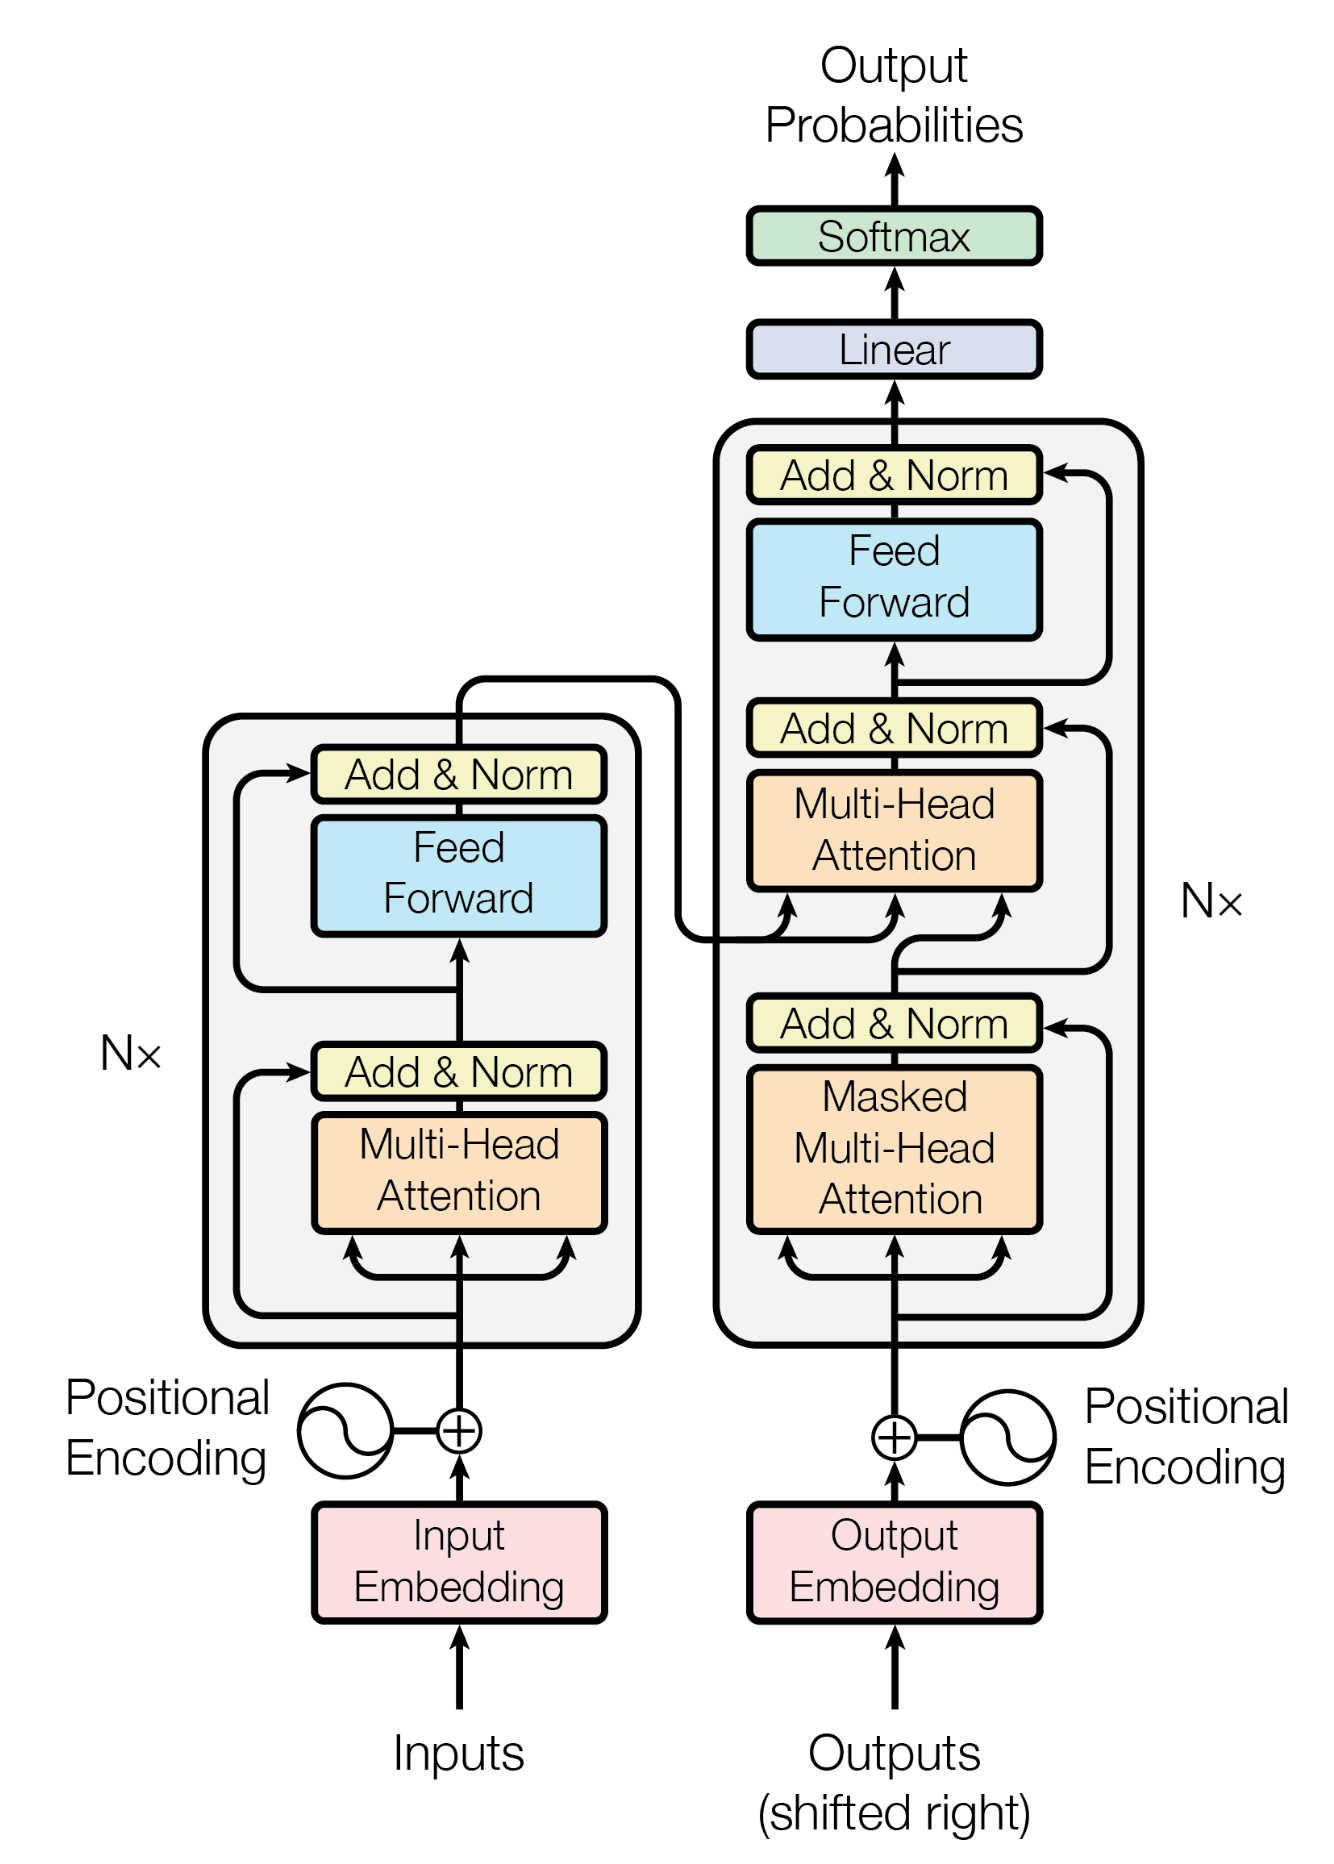
\includegraphics[width=0.39\textwidth]{figures/transformer_model_architecture.png}
        \end{center}
    \end{wrapfigure}
    
    
    \subsection{BERT}
    \label{sec:-bert}

        \textbf{B}idirectional \textbf{E}ncoder \textbf{R}epresentation from \textbf{T}ransformer, often abbreviated to BERT heavily relies on the concept of \emph{Attention} and the usage of \emph{Transformers} that are presented in the famous paper "Attention is All You Need"\cite{vaswani2017attention}.
        Inside the ML-model, there is a multilayer bidirectional transformer encoder structure, hence the name of BERT and in general it is differentiated between two types of BERT models, that are named BERT$_{Base}$ and BERT$_{Large}$.
        The BERT$_{Base}$ model has 12 layers of transformer blocks, a hidden size of $768$ and 12 self-attention heads as well as 110 million trainable parameters. \textbf{Note: This is the model type I used in this project.}

        BERT$_{Large}$ is even bigger, using $24$ layers of transformer blocks and has a hidden size of $1024$, it uses 16 self-attention heads and has $340$ million trainable parameters. This of course is too big for a regular computing device to retrieve a feasible result.

                
\pagebreak
    \section{Implementation}
    \label{sec:implementation}
            
            Transformers is responsible for downloading the machine learning model \texttt{BERT}.
            \texttt{BERT} is short for \emph{Bi}

    % Implementation: how did you implement your approach? which tools were used? show interesting snippets or present your algorithms.

        Placeholder

    \section{Evaluation}
    \label{sec:evaluation}

    % Evaluation: present and visualize results of your evaluation, explain what do your results mean, why was your approach successful, why not? compare it to some baseline either implemented yourself or from the literature, blogs, Kaggle, etc.
        Placeholder

    \section{Conclusion}
    \label{sec:conclusion}
    % Conclusions: how can you evaluate the results of your work? what would you recommend for future steps?

        Placeholder

    \section{Supplementary Materials}
    \label{sec:supplementary-materials}

        owijfgiowjeiofjio

    % Supplementary materials: The report must be submitted as an archive comprising all code and artifacts (data, custom python modules, images, videos, etc.) required for its correct representation, evaluation, and exemplification of your work. If data is too large for a submission, please provide a link where this data can be downloaded from.

    \pagebreak

    \bibliography{references.bib}
    \bibliographystyle{ieeetr}
    % \printbibliography

\end{document}
